\documentclass[10.5pt, stu, hidelinks, noendfloat]{apa7}

% Paquets de llengua i codificació
\usepackage[T1]{fontenc}
\usepackage[catalan]{babel}

% Configuració de Citacions en estil APA 7
\usepackage[style=apa, backend=biber]{biblatex}
\addbibresource{export.bib} % bibliografia

% Activar la numeració de seccions a apa7
\setcounter{secnumdepth}{3}

% Fonts
\usepackage{newtxtext}
\usepackage{newtxmath}

% Grafiques
\usepackage{graphicx}
\usepackage{float}

\title{Repte 1: IA per a jocs en primera persona}
\author{Iris Garcia Gomez}
\course{M7.459 - Intel·ligència artificial per a videojocs}
\professor{Professorat: Gerard Escudero Bakx}
\duedate{\today}
\authorsaffiliations{Universitat Oberta de Catalunya UOC}

\begin{document}

\clearpage
\maketitle
\clearpage

\section*{Enllaços:}
\begin{enumerate}
\item Repositori de GitHub: \href{https://github.com/burbuuu/IA-Repte1}{Repositori}
\item Activitat 2: \href{https://youtu.be/oTkYbqyRmkw}{Wander}
\item Activitat 3: \href{https://youtu.be/TVM16daaVkM}{Patrol i Flee}
\end{enumerate}

\section{Activitat 1: Escenari}
Per a aquesta activitat he partit del paquet d'assets \href{https://assetstore.unity.com/packages/3d/environments/fantasy/polygonal-fantasy-cemetery-stylized-low-poly-art-150116}{Polygonal Fantasy Cemetery}, del qual dispose de la llicència corresponent. A partir de l'escena de demostració, amb l'objectiu de d'aprofitar la il·luminació i l'estructura, he dissenyat un cementeri. 

Finalment, he integrat i generat la \textit{Nav Mesh}, limitant les seues dimensions al interior del cementeri.

\begin{center}
    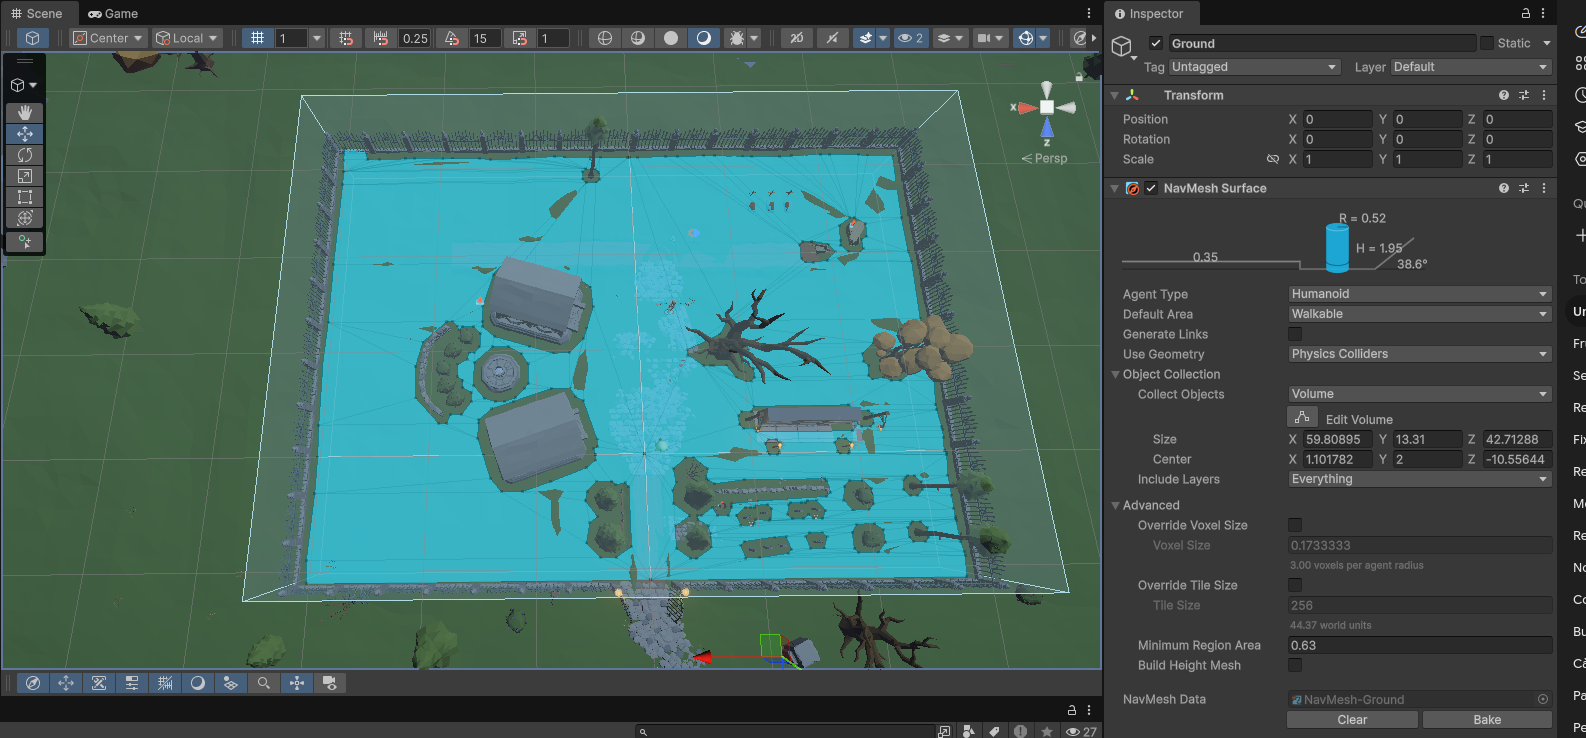
\includegraphics[width=\textwidth]{images/NavMesh.png}
    \vspace{0.2cm}
    \captionof{figure}{Vista de la configuració de la NavMesh.}
    \label{fig:navmesh_cemetery}
\end{center}


\section{Activitat 2: Wander}

Per a aquesta activitat he utilitzat el model i les animacions del paquet d'assets \href{https://assetstore.unity.com/packages/3d/characters/creatures/ghost-cute-series-162548}{Ghost Cute Series}, del qual dispose de la llicència corresponent.

Primerament, s'ha implementat l'algorisme suggerit als apunts (GitHub de l'assignatura), adaptat al \textit{Visual Scripting} i a l'ús del sistema \textit{Nav Mesh} de Unity. 

El primer pas es crear un loop, que permeta controlar la freqüència de càlcul de direcció del personatge. Es construeix a traves de la corutina \textit{Wait For Seconds}. Veure la figura \ref{fig:loop}. 


\begin{center}
    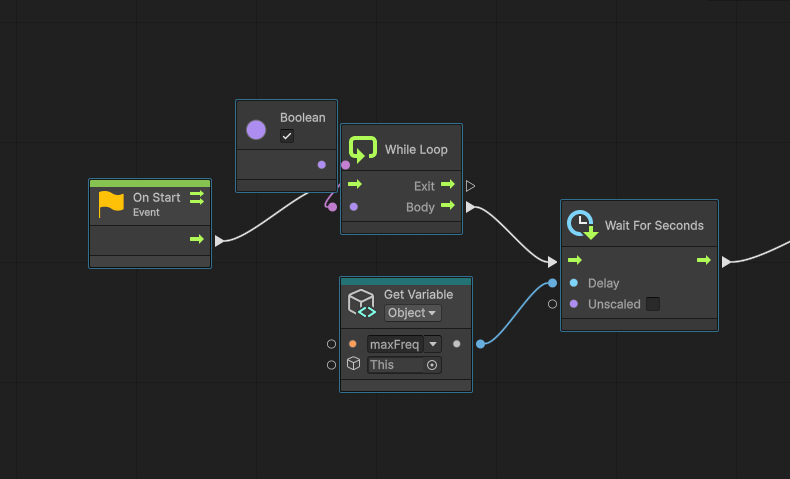
\includegraphics[width=0.7\textwidth]{images/Loop.png}
    \vspace{0.2cm}
    \captionof{figure}{Wander 1: Loop construit a partir de la corutina \textit{Wait For Seconds}.}
    \label{fig:loop}
\end{center}

\begin{center}
    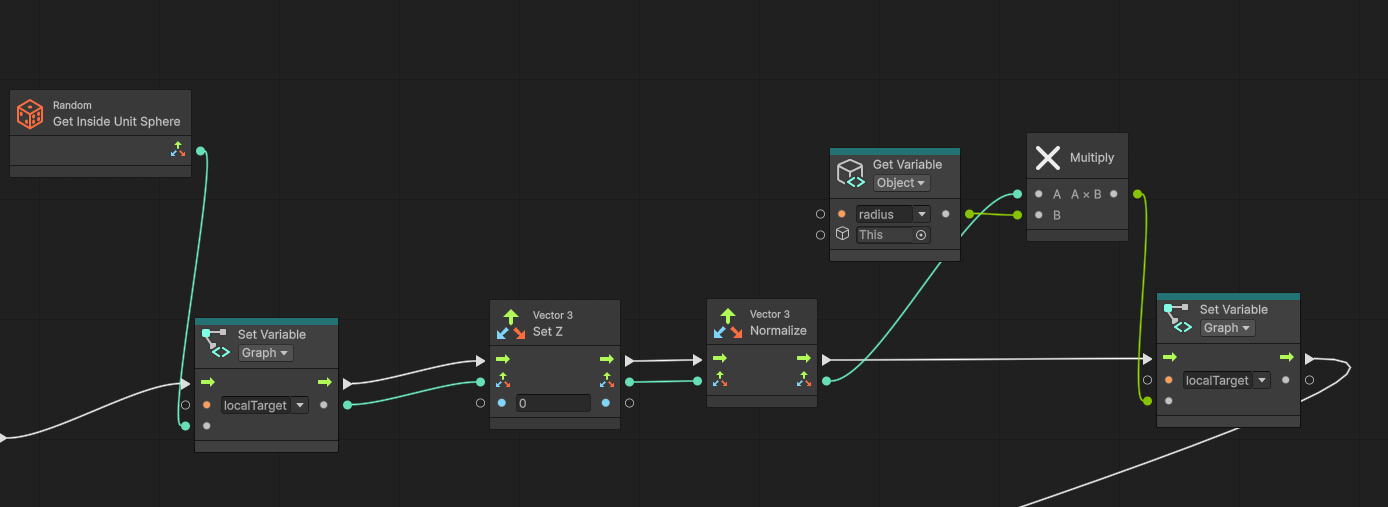
\includegraphics[width=\textwidth]{images/Wand2.png}
    \vspace{0.2cm}
    \captionof{figure}{Wander 2: Creació del local target a partir d'una esfera de radi $r$.}
    \label{fig:wand2}
\end{center}


Durant les proves, he observat que al tenir una superfície limitada (un area rectangular), quan l'agent es troba a una vora i l'\textit{offset} és més gran que el radi de l'esfera (element aleatori), l'agent es queda atascat al cantó. 
La solució aplicada a aquest problema, pasa per veure si l'offset queda fora de la \textit{NavMesh}, i si és el cas es multiplica per un factor negatiu ($\tau \sim -0.3$), guiant l'agent cap a l'interior de l'area. 

\begin{center}
    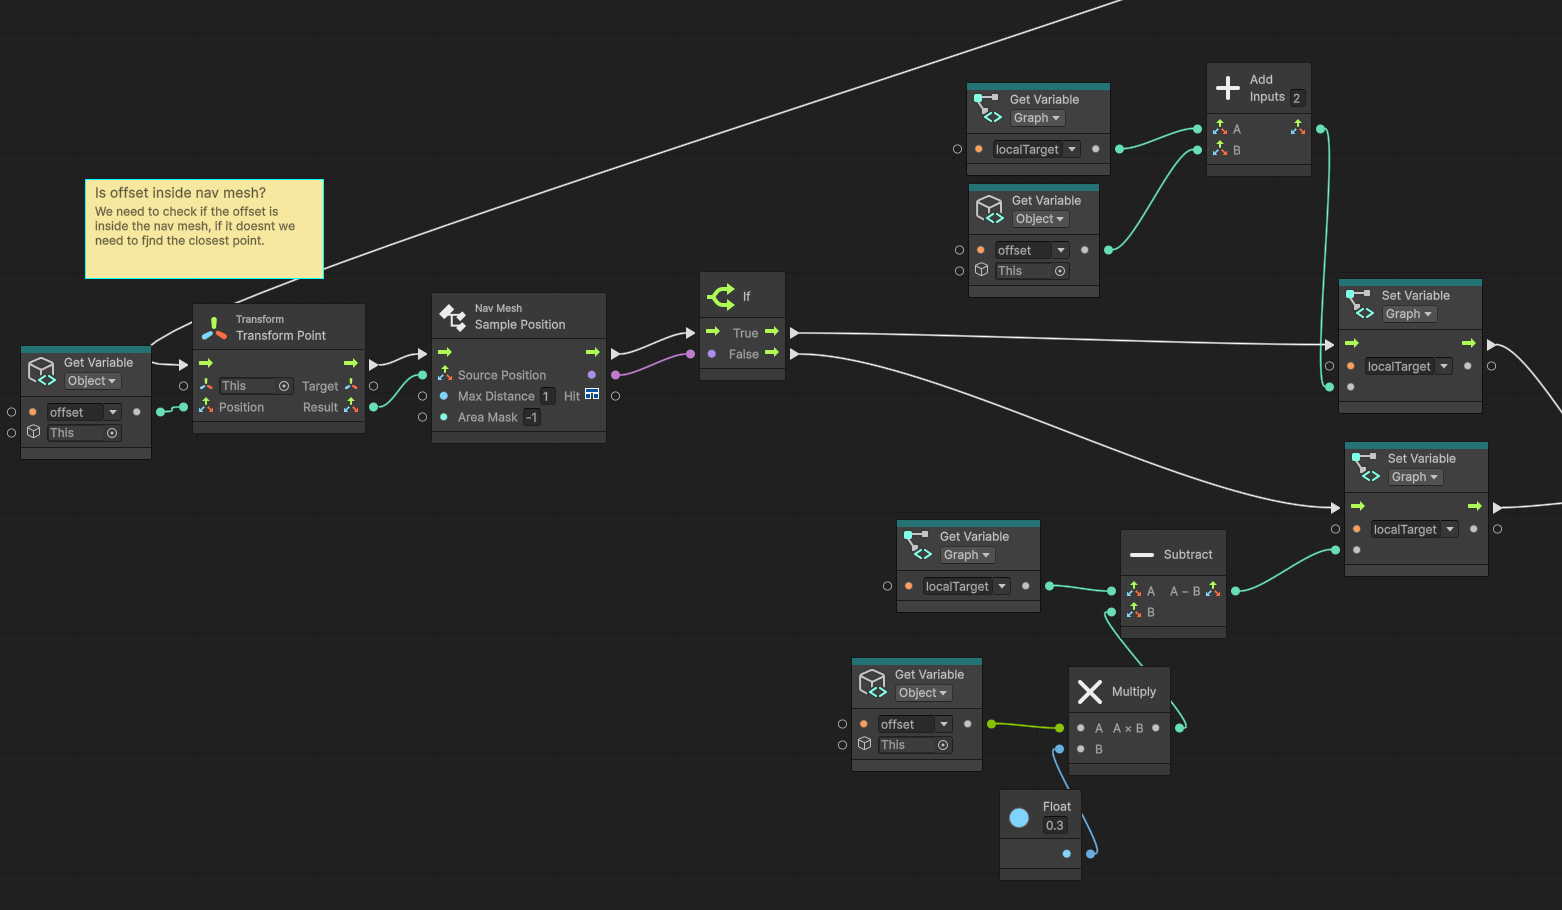
\includegraphics[width=\textwidth]{images/OffsetCheck.png}
    \vspace{0.2cm}
    \captionof{figure}{Wander 3: Comprovació del offset, si aquest cau fora de la \textit{NavMesh}, s'aplica un factor de correció negatiu.}
\end{center}

Finalment es defineix el nou destí.

\begin{center}
    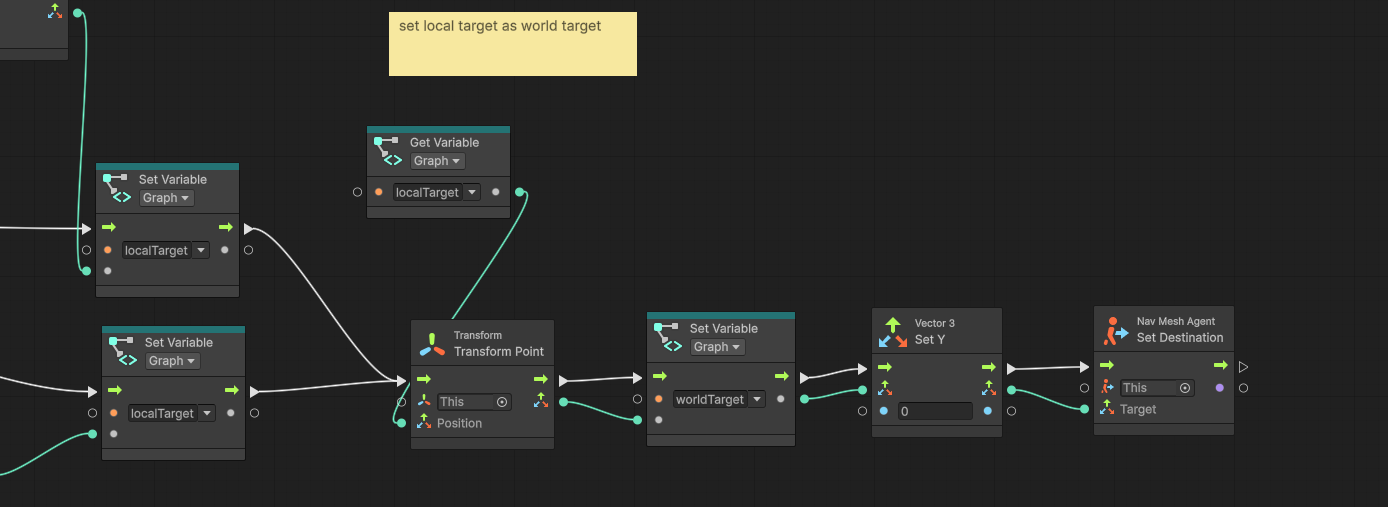
\includegraphics[width=\textwidth]{images/Wand4.png}
    \vspace{0.2cm}
    \captionof{figure}{Wander 4: Assignació de camí per a l'agent.}
    \label{fig:wand4}
\end{center}

\subsection{Demostració}
Al video es pot observar el resultat del moviment.\href{https://youtu.be/oTkYbqyRmkw}{\textit{Enllaç a vídeo demostració.}}



\section{Activitat 3: Patrol i Flee}

Per a l'agent programat en aquesta activitat s'ha escollit un esquelet del paquet \textit{Polygonal Fantasy Cemetery} amb animacions d'us lliure de \textit{Mixamo}. L'agent s'ha implementat utilitzant un \textit{State Graph} que representa la màquina d'estats.

\begin{center}
    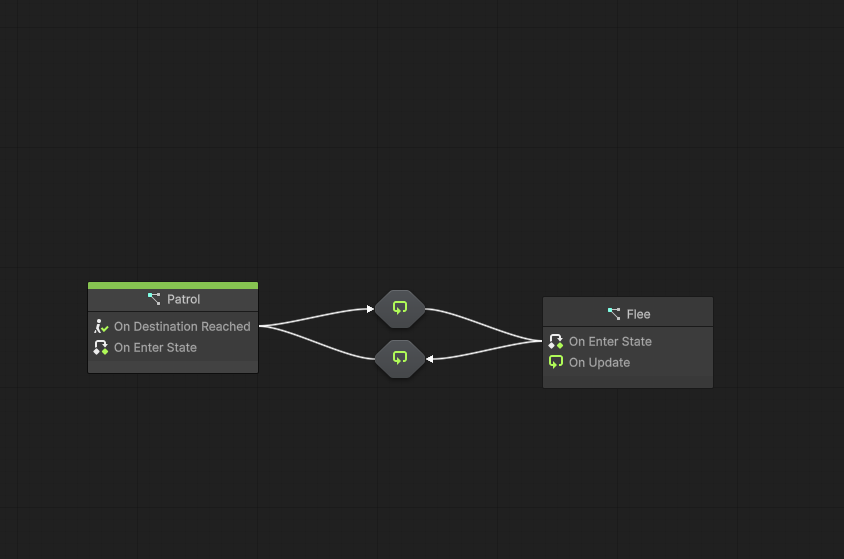
\includegraphics[width=0.7\textwidth]{images/FSM.png}
    \vspace{0.2cm}
    \captionof{figure}{Maquina d'estats de l'agent.}
    \label{fig:FSM}
\end{center}

\subsection{Patrol:}

Entrada de l'estat:

\begin{center}
    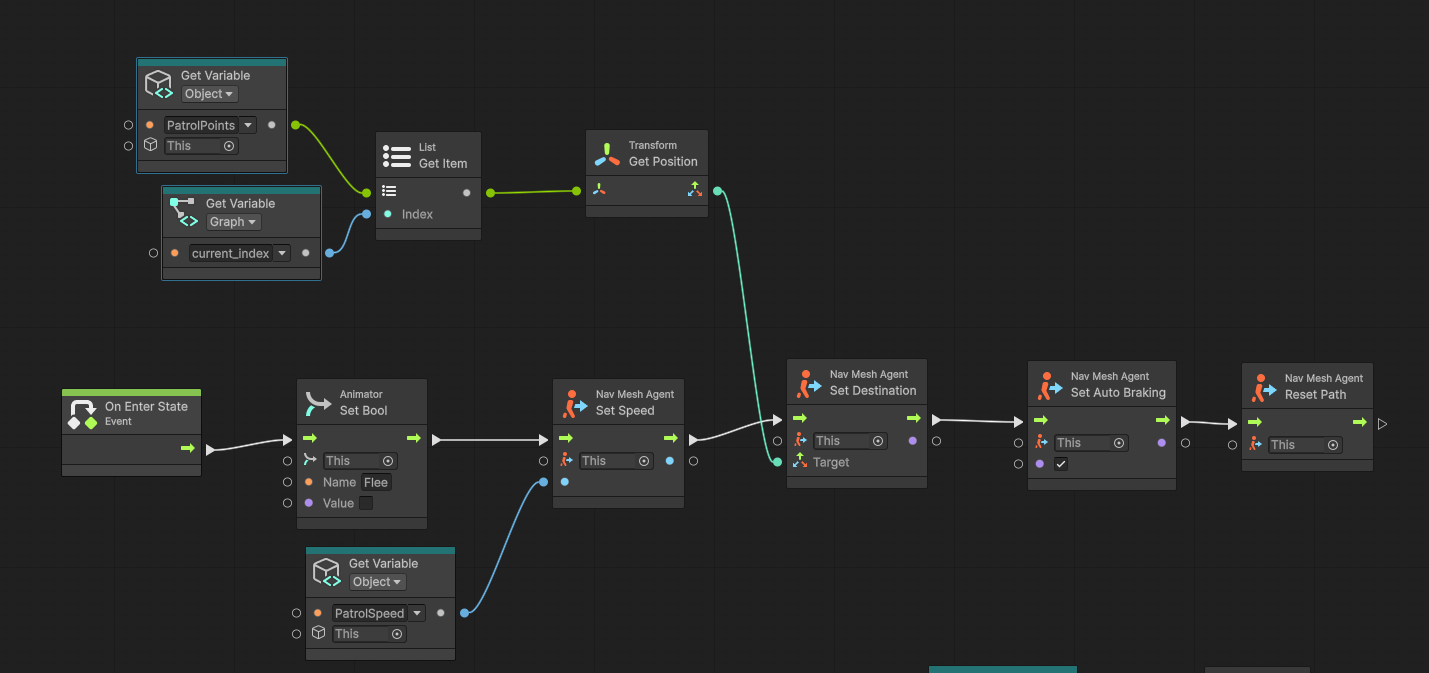
\includegraphics[width=\textwidth]{images/Patrol1.png}
    \vspace{0.2cm}
    \captionof{figure}{\textbf{On Enter:} Selecció de velocitat de patrol i reinici de camí de l'agent.}
    \label{fig:Patrol1}
\end{center}

\textit{Loop} principal de l'estat:

\begin{center}
    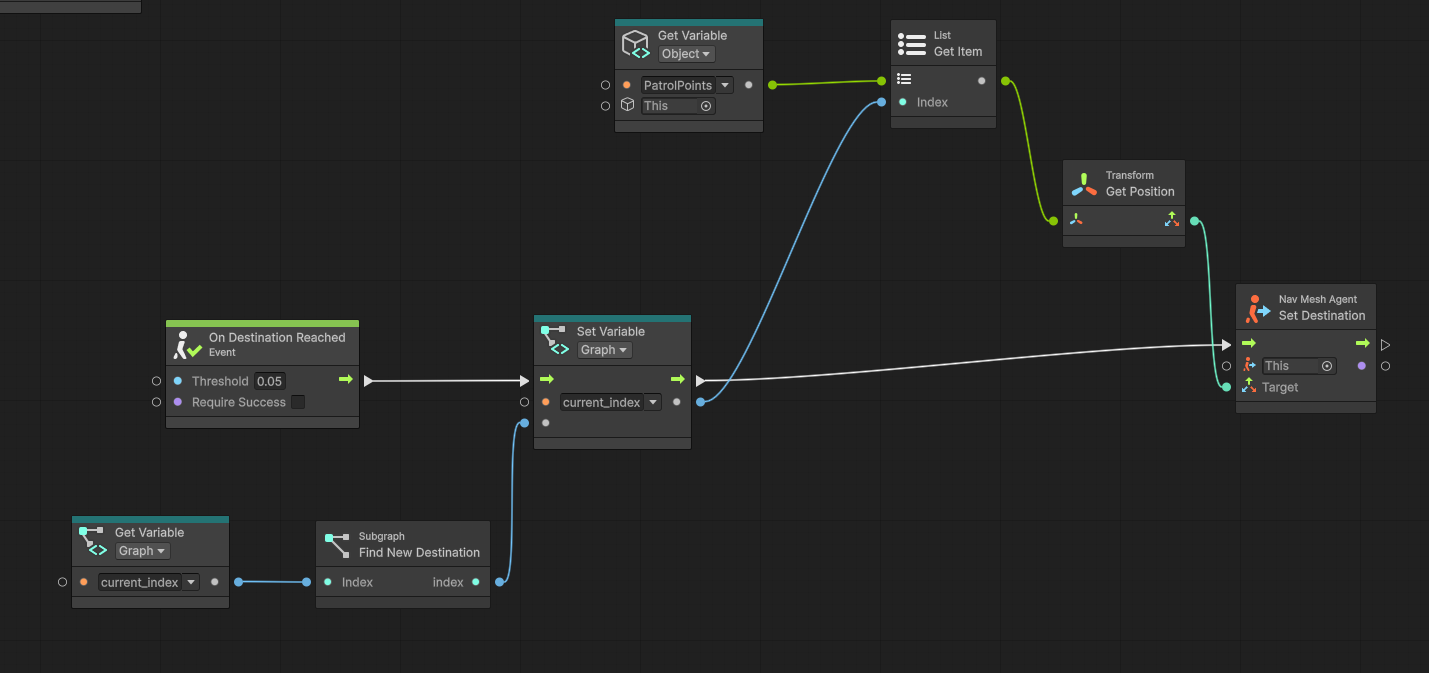
\includegraphics[width=\textwidth]{images/Patrol2.png}
    \vspace{0.2cm}
    \captionof{figure}{\textbf{Update:} Selecció d'un nou destí.}
    \label{fig:Patrol2}
\end{center}

Com es pot observar a \ref{fig:Patrol2}, s'utilitza un \textit{subgraph} per calcular l'índex del nou destí.

\begin{center}
    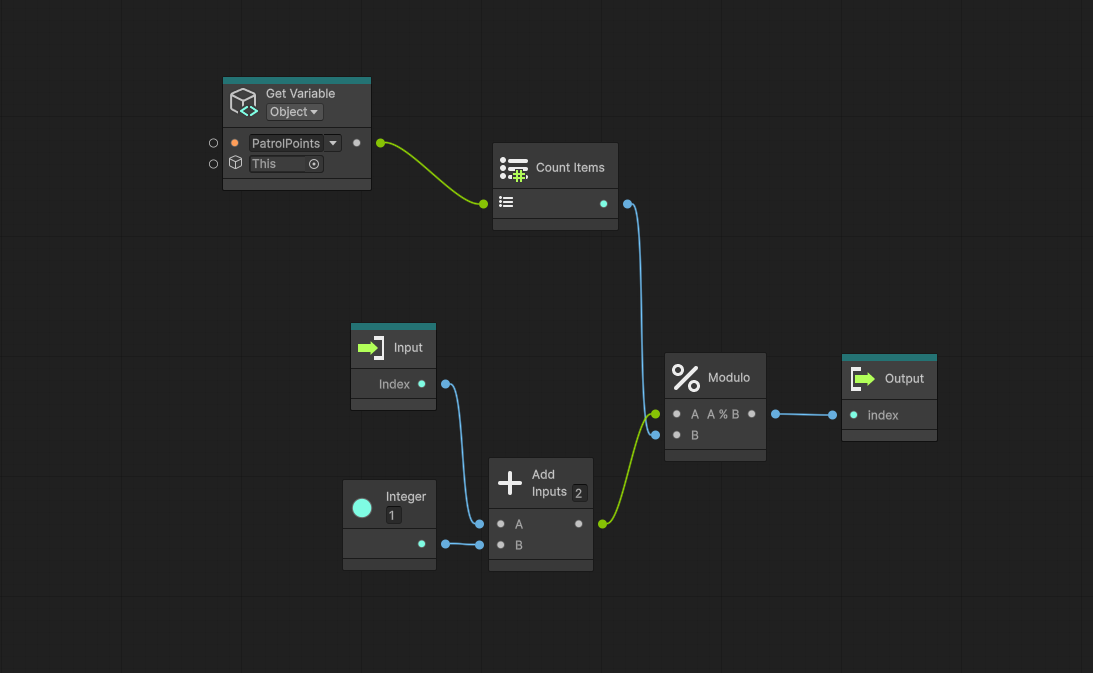
\includegraphics[width=\textwidth]{images/Patrol3.png}
    \vspace{0.2cm}
    \captionof{figure}{\textbf{Subgraph:} Ús del mòdul per calcular el nou index.}
    \label{fig:Patrol3}
\end{center}


\subsection{Flee}

Primerament s'assignen els parametres de moviment a l'agent i s'activen les animacions:
\begin{center}
    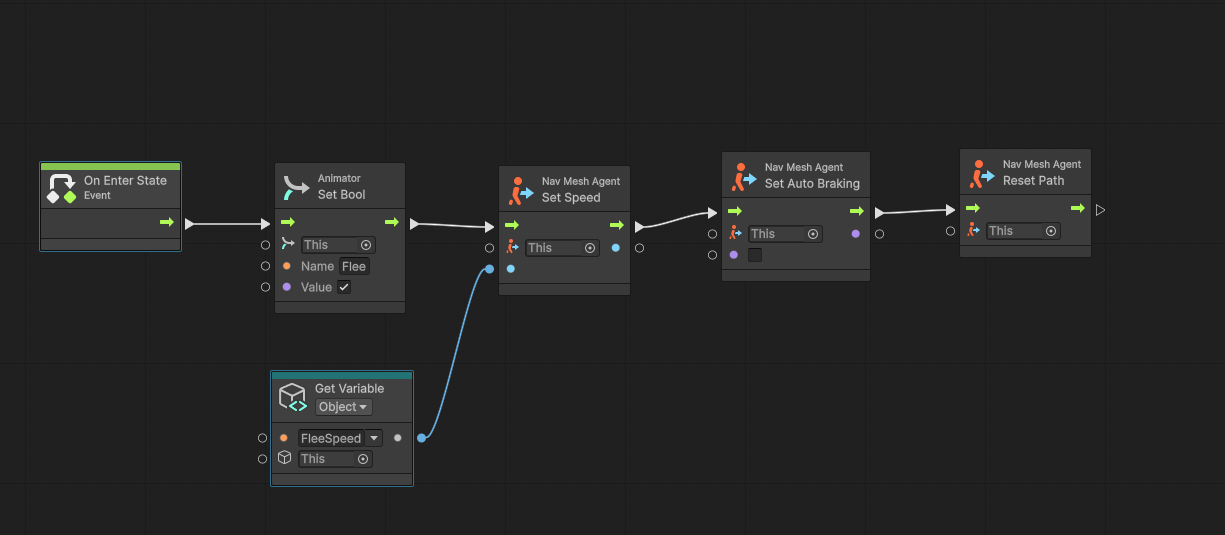
\includegraphics[width=\textwidth]{images/Flee1.png}
    \vspace{0.2cm}
    \captionof{figure}{\textbf{On Enter:} Selecció de velocitat de \textit{flee} i reinici de camí de l'agent.}
    \label{fig:Flee1}
\end{center}

Igual que al wander, s'utilitza un bucle \ref{fig:loop} per limitar quantes voltes es calcula el camí per segon. Tot seguit es calcula la direcció el nou camí:

\begin{center}
    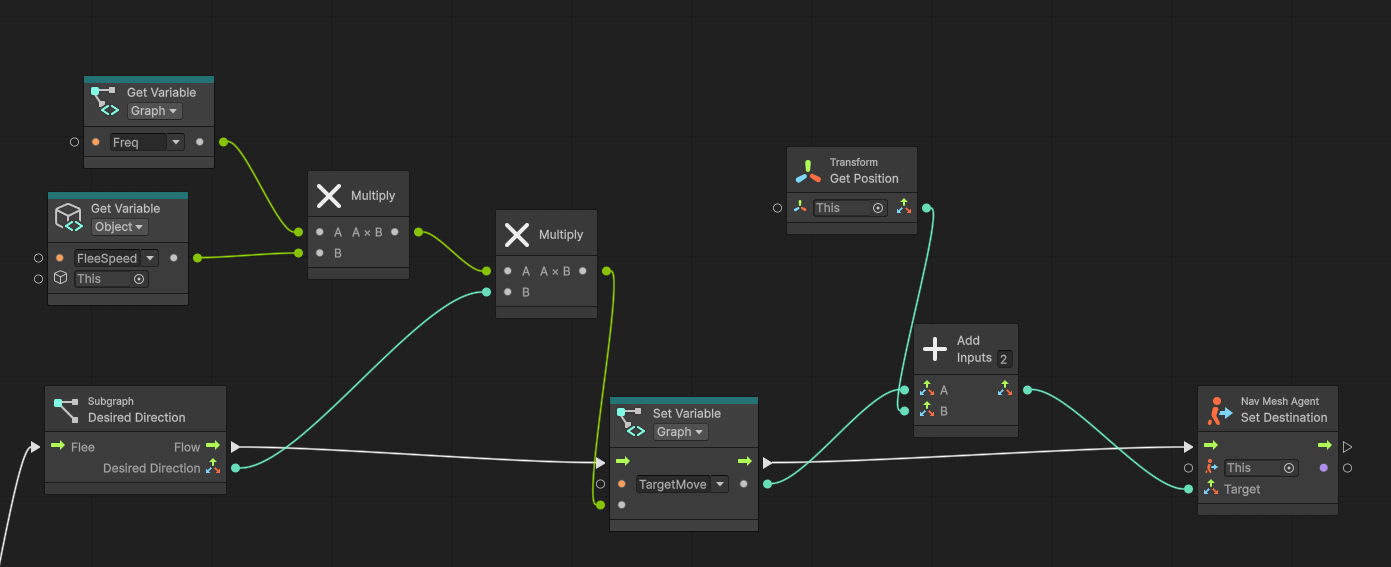
\includegraphics[width=\textwidth]{images/Flee2.png}
    \vspace{0.2cm}
    \captionof{figure}{\textbf{Update:} Càlcul del nou camí, evitant el fantasma (\textit{target}). La direcció de fugida es calcula al subgràfic \textit{Desired Direction}. Amb aquesta direcció i la velocitat (\textit{speed}) de l'agent es calcula el nou destí.}
    \label{fig:Flee2}
\end{center}

Per calcular la direcció desitjada s'utilitza tant la posició, com la velocitat i direcció de moviments desitjades del \textit{target.} Es fa una estimació de la trajectoria aproximada de l'agent, i es s'inverteix aquesta direcció per tal de fugir de forma eficient. Figures \ref{fig:Flee3} i \ref{fig:Flee4}.
\begin{center}
    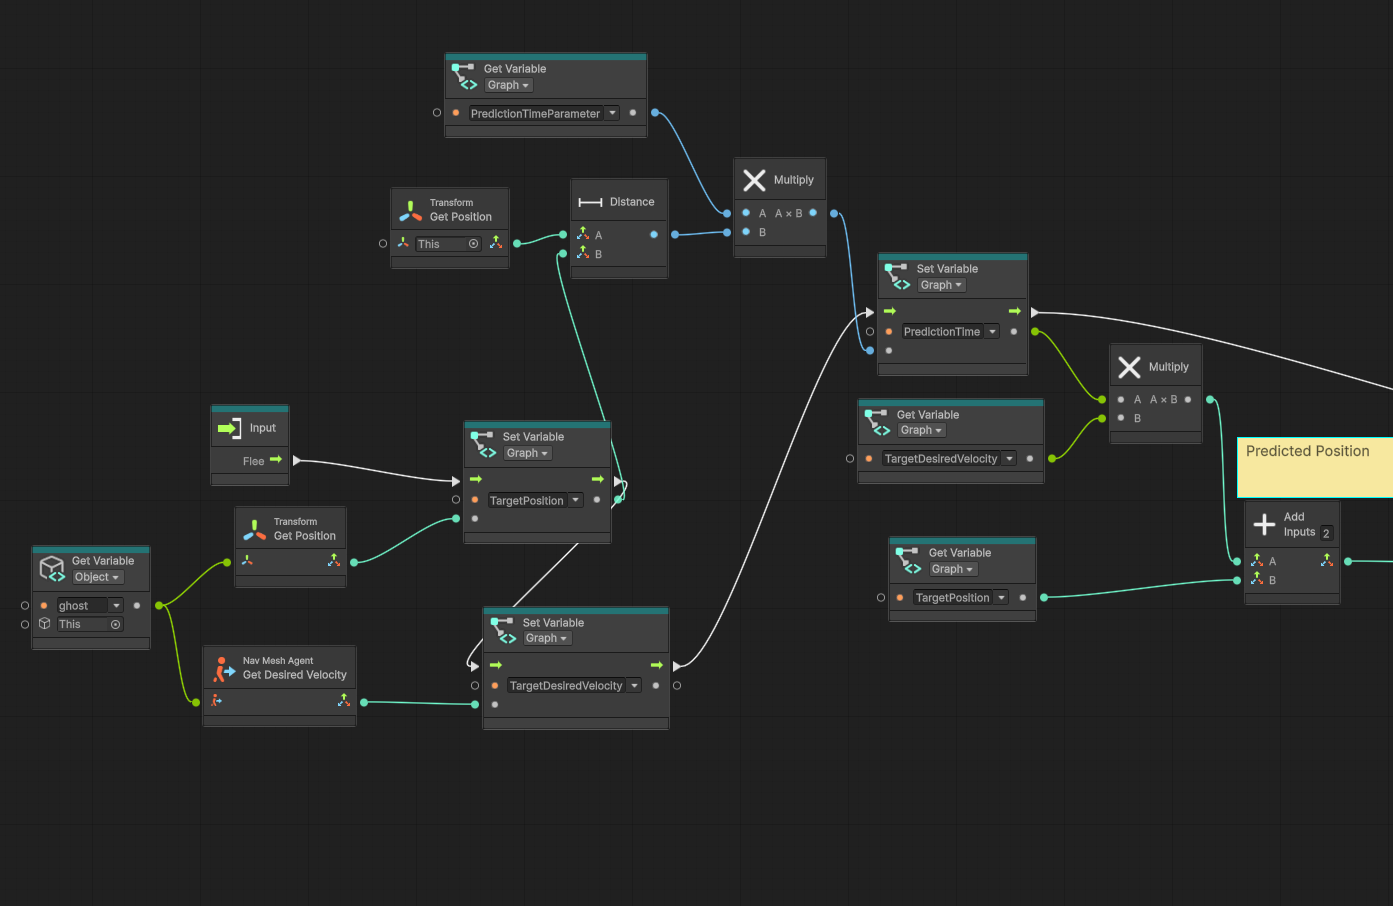
\includegraphics[width=\textwidth]{images/Flee3.png}
    \captionof{figure}{Detall de càlcul de la direcció de fugida (part 1).}
    \label{fig:Flee3}
\end{center}

\begin{center}
    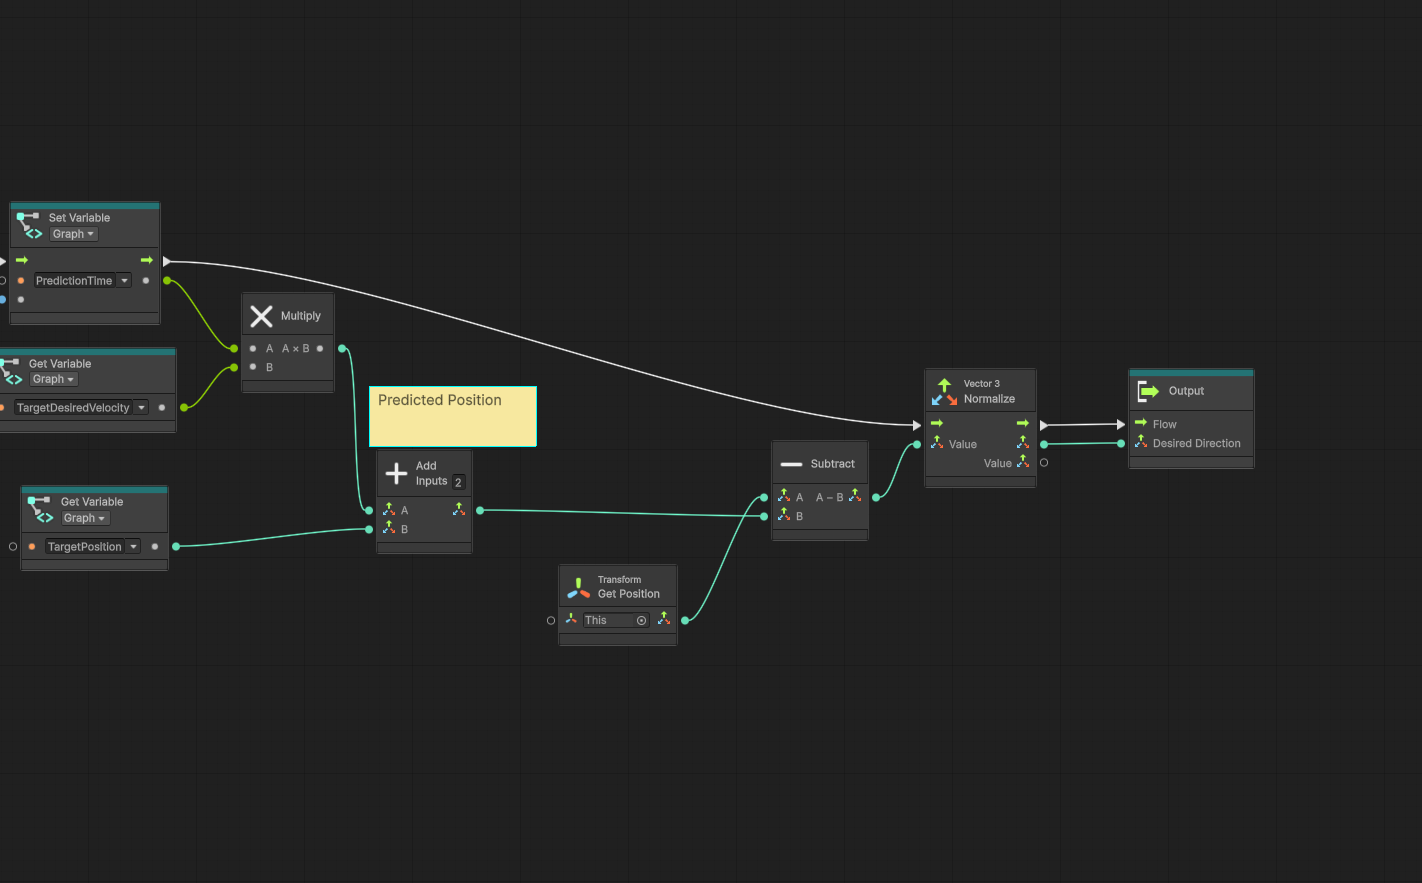
\includegraphics[width=\textwidth]{images/Flee4.png}
    \captionof{figure}{Detall de càlcul de la direcció de fugida (part 2).}
    \label{fig:Flee4}
\end{center}

\subsection{Transicions d'estat.}
 Les transicions d'estat s'han calculat mitjançant dos distàncies:
 
 \begin{center}
    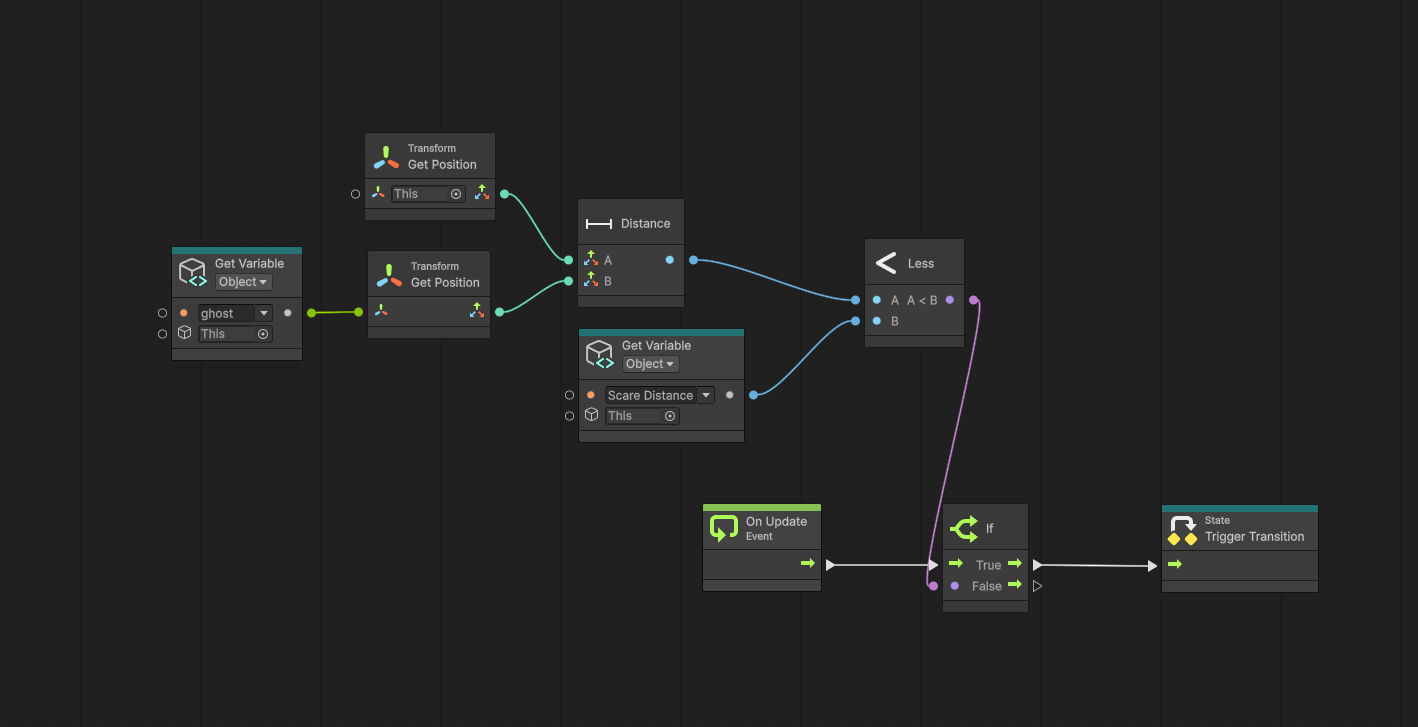
\includegraphics[width=\textwidth]{images/PatrolToFlee.png}
	\captionof{figure}{Transició de l'estat de patrol a flee basada en la proximitat de l'objectiu.}   
 	\label{fig:trans1}
\end{center}
\begin{center}
    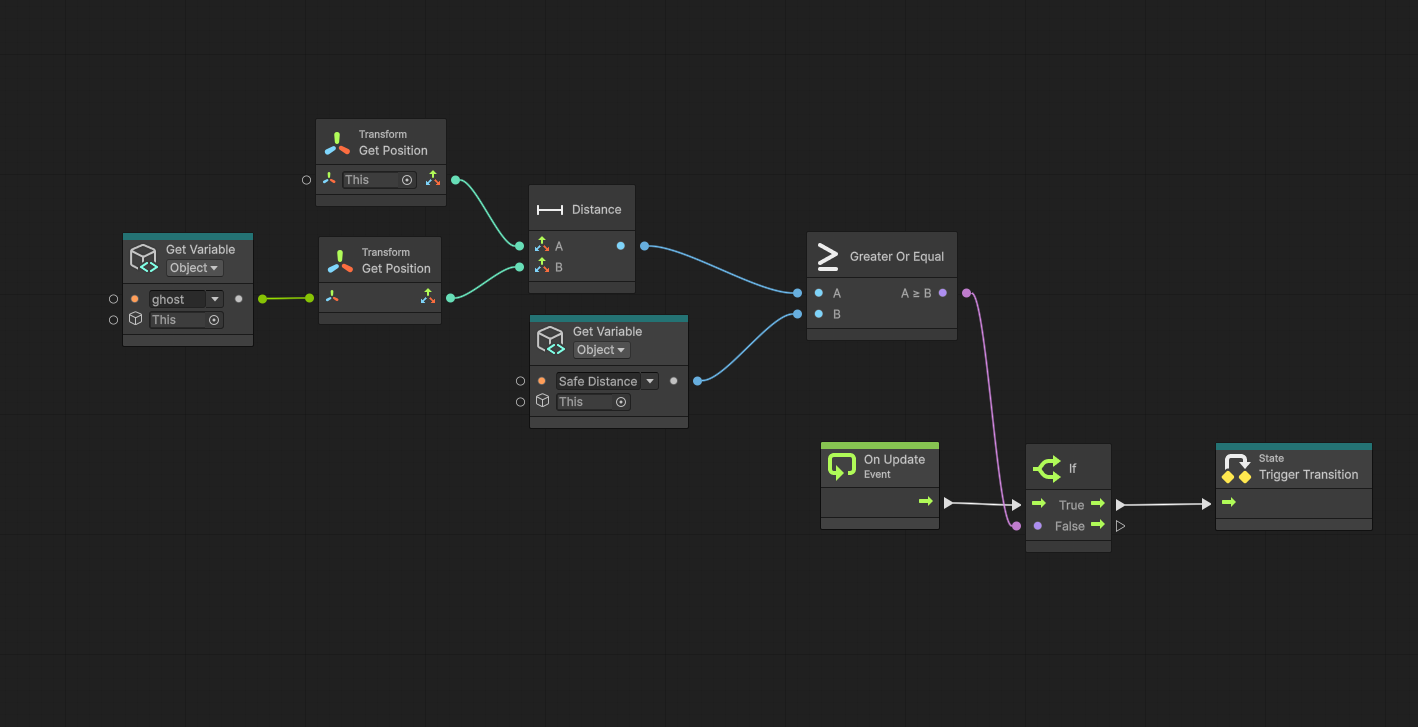
\includegraphics[width=\textwidth]{images/FleeToPatrol.png}
	\captionof{figure}{Transició de l'estat de flee a patrol en augmentar la distància respecte al fantasma.}
    \label{fig:trans2}
\end{center}



\subsection{Demostració}

Al video es pot observar el resultat del moviment: \href{https://youtu.be/TVM16daaVkM}{Patrol i Flee}


\section{Ús de l'inteligencia artíficial}

En aquest treball s'ha utilitzat inteligencia artificial per cobrir la falta de documentació d'alguns nodes de \textit{Visual Scripting} de Unity. Ha resultat una eina útil per aprendre el funcionament d'alguns nodes específics com: \textit{NavMesh Path Status}, o \textit{NavMesh Sample Position}. 
Aquesta pregunta: "Why the literal "Path completed" (on a visual scripting node on Unity, for a nav mesh agent), does not represent if the agent have finished the their path? " amb el xat Gemini, em va ajudar a depurar un error al codi on verificava si l'agent \textit{wander} podia acabar el seu camí.
En aquest cas, l'ús de la IA, ha estat d'una útilitatgit límitada, per cobrir una documentació incompleta per part d'Unity.


\end{document}